\PassOptionsToPackage{obeyspaces,spaces}{url}
\documentclass[11pt,a4paper]{article}
\usepackage[margin=2.1cm]{geometry}
\usepackage{amsmath,amssymb}
\usepackage{graphicx}
\usepackage{booktabs,tabularx,longtable,array}
\usepackage{xcolor}
\usepackage{float}
\usepackage{caption}
\usepackage{listings}
\usepackage{tikz}
\usetikzlibrary{arrows.meta,positioning}
\usepackage{xurl}
\usepackage[colorlinks=true,linkcolor=blue!50!black,urlcolor=blue!50!black]{hyperref}
\urlstyle{tt}
\newcommand{\code}[1]{\nolinkurl{#1}}
\newcolumntype{L}[1]{>{\raggedright\arraybackslash}p{#1}}

\lstdefinestyle{py}{language=Python,basicstyle=\ttfamily\scriptsize,breaklines=true,columns=fullflexible,
  frame=single,backgroundcolor=\color{gray!6},keywordstyle=\color{blue!60!black}\bfseries,
  commentstyle=\color{green!40!black},stringstyle=\color{red!50!black},numbers=left,numberstyle=\tiny\color{gray},
  showstringspaces=false,keepspaces=true}
\lstdefinestyle{sh}{basicstyle=\ttfamily\small,breaklines=true,columns=fullflexible,frame=single,
  backgroundcolor=\color{gray!6},showstringspaces=false,keepspaces=true}
\lstset{style=sh}
% \src{file relative to unlearnable_games_explanation}{first}{last}{caption}
\newcommand{\src}[4]{\lstinputlisting[style=py,firstline=#2,lastline=#3,firstnumber=#2,
  title={\footnotesize\code{#1}, lines #2--#3: #4}]{../../unlearnable_games_explanation/#1}}

\title{How the project uses D-Wave\\[4pt]\large Code walk-through, modes of use, checks, estimates, budget guard, and the 1-second test}
\author{\code{Projects_master_HPQC/scripts/QuantumComputing/Dimod}}
\date{}

\begin{document}
\maketitle
\begin{abstract}
This document explains, file by file and line by line, how the SK-game campaign talks to D-Wave:
\begin{itemize}
\item which Ocean functions it uses, what they can do, and how the code harnesses them;
\item the six ways (``modes'') of running an annealer in this project;
\item what \code{qpu --check} actually does, and how the QPU time is estimated (three levels, with the formulas);
\item how the budget guard (\code{--budget-seconds}) makes sure a run never exceeds a given QPU time;
\item how the results are turned into success probabilities, time-to-solution and the Zephyr/Pegasus comparison.
\end{itemize}
The code excerpts are read directly from the source files when the document is compiled, so the line numbers
are those of the version in the repository. Section~\ref{sec:plan} gives the exact commands for a test
that uses at most one second of QPU time, followed by a plan to spend the 180 s of this month before 4 November.
\end{abstract}
\tableofcontents
\newpage

%=====================================================================================
\section{Where the D-Wave code lives}
%=====================================================================================
All paths are relative to \code{Dimod/src/unlearnable_games_explanation/}.

\begin{table}[H]\centering\small
\begin{tabularx}{\linewidth}{L{5.0cm}X}
\toprule
file & role \\ \midrule
\code{skgame/optim/problem.py} & the SK problem $W$; \code{to_bqm()} builds the dimod model \\
\code{skgame/optim/embedding.py} & topologies (Zephyr, Pegasus), embedding strategies (clique, heuristic), chain statistics, embedding cache \\
\code{skgame/optim/backends.py} & \code{AnnealBackend}: one object per \code{device:topology:strategy}; builds the sampler, embeds, samples, collects statistics, estimates time \\
\code{skgame/optim/quantum.py} & \code{QuantumAnnealingSolver}: the older single-solver path (\code{DWaveCliqueSampler}/\code{EmbeddingComposite}), used by the planner benchmark \\
\code{skgame/optim/solvers.py} & \code{DimodSamplerSolver} (generic dimod wrapper) and the classical dimod samplers \\
\code{main_simulation.py} & the campaign: stages \code{init}, \code{instances}, \code{classical}, \code{embed}, \code{qpu}/\code{sim}, \code{analyze}; the QPU budget guard; the analysis \\
\code{tests/test_embedding.py}, \code{tests/test_campaign.py} & tests of all the above, including the QPU path against D-Wave's mock QPU \\
\bottomrule
\end{tabularx}
\end{table}

\begin{figure}[H]\centering
\begin{tikzpicture}[node distance=0.5cm and 0.45cm,
  box/.style={draw,rounded corners,fill=blue!6,align=center,font=\scriptsize,minimum height=1cm,text width=2.45cm},
  arr/.style={-{Stealth},thick}]
\node[box] (cli) {\code{main_simulation.py qpu}\\(\code{main})};
\node[box,right=of cli] (st) {\code{stage_anneal}\\budget guard};
\node[box,right=of st] (be) {\code{AnnealBackend}\\\code{.sample(P)}};
\node[box,right=of be] (emb) {\code{EmbeddingCache}\\\code{CliqueEmbedding}};
\node[box,below=of emb] (fec) {\code{FixedEmbeddingComposite}\\chain strength, breaks};
\node[box,left=of fec] (dws) {\code{DWaveSampler}\\(Leap, SAPI)};
\node[box,left=of dws] (stat) {\code{sampleset_statistics}\\rewards, timing, polish};
\node[box,left=of stat] (json) {\code{anneal/<backend>/}\\\code{...json}};
\draw[arr] (cli)--(st); \draw[arr] (st)--(be); \draw[arr] (be)--(emb); \draw[arr] (emb)--(fec);
\draw[arr] (fec)--(dws); \draw[arr] (dws)--(stat); \draw[arr] (stat)--(json);
\end{tikzpicture}
\caption{The path of one QPU call through the code.}
\end{figure}

%=====================================================================================
\section{The Ocean SDK: what each package can do, and what we use it for}
%=====================================================================================
D-Wave's Python SDK (\emph{Ocean}) is a set of packages, all installed by \code{cineca/requirements.txt}.
For each package: what it offers, then exactly how this project uses it.

\subsection{\texorpdfstring{\code{dwave-cloud-client}}{dwave-cloud-client}: connection, solvers, configuration, timing model}
\textbf{Capabilities.}
\begin{itemize}
\item it talks to the Leap \emph{Solver API} (SAPI) over HTTPS;
\item it reads the token from the configuration file or from the environment (\code{DWAVE_API_TOKEN});
\item it selects solvers with \emph{feature filters} such as \code{solver={"topology__type": "zephyr"}};
\item it exposes every solver's \code{properties}, including the timing data;
\item it estimates the cost of a problem (\code{estimate_qpu_access_time});
\item it submits problems asynchronously;
\item it provides the \code{dwave} command line: \code{config}, \code{auth}, \code{leap}, \code{solvers}, \code{ping}, \code{setup}.
\end{itemize}

\textbf{How we use it.}
\begin{itemize}
\item Through \code{DWaveSampler} (next subsection), which wraps a cloud-client \code{Solver}.
\item \code{solver.name} identifies the QPU in the logs and keys the embedding cache, e.g.\ \code{Advantage2_system1}.
\item \code{solver.estimate_qpu_access_time} is the second level of our time estimate (\S\ref{sec:estimate}).
\item On the command line: \code{dwave config create}, \code{dwave setup --oob}, \code{dwave solvers -la}, \code{dwave ping} (\code{Dimod/LEAP_TOKEN.md}).
\end{itemize}

\subsection{\texorpdfstring{\code{dwave-system}}{dwave-system}: samplers for the QPU, composites, mock}
\textbf{Capabilities.}
\begin{itemize}
\item \code{DWaveSampler}: a dimod sampler bound to one structured QPU. It exposes \code{nodelist}/\code{edgelist} (the working qubits and couplers), \code{properties}, \code{parameters} (the accepted keyword arguments) and \code{to_networkx_graph()}. Its \code{sample()} accepts \code{num_reads}, \code{annealing_time}, \code{anneal_schedule}, \code{auto_scale}, \code{answer_mode}, \code{h_gain_schedule}, \code{anneal_offsets}, \code{programming_thermalization}, \code{readout_thermalization}, \dots
\item Composites that turn a structured sampler into one that accepts any problem:
\begin{itemize}
\item \code{EmbeddingComposite} finds a heuristic embedding on every call;
\item \code{FixedEmbeddingComposite} uses a given embedding;
\item \code{LazyFixedEmbeddingComposite} finds one embedding and reuses it;
\item \code{DWaveCliqueSampler} uses cached all-to-all clique embeddings, scales with the extended $J$ range and computes chain strengths.
\end{itemize}
\item \code{dwave.system.testing.MockDWaveSampler}: an offline imitation of a QPU of any topology and size, which returns realistic timing fields.
\end{itemize}

\textbf{How we use it.}
\begin{itemize}
\item \code{DWaveSampler(solver={"topology__type": ...})} picks a Zephyr or Pegasus QPU (code below).
\item \code{to_networkx_graph()} gives the \emph{real} working graph. The embedding is computed on it, so it avoids dead qubits.
\item Every QPU call goes through \code{FixedEmbeddingComposite} with our cached clique embedding. The Zephyr and Pegasus back-ends then go through identical code and differ only in hardware and embedding.
\item \code{DWaveCliqueSampler} and \code{EmbeddingComposite} remain available in \code{QuantumAnnealingSolver} (\S\ref{sec:modes}).
\item \code{MockDWaveSampler} is used in the tests and in the dry runs.
\end{itemize}

\src{skgame/optim/backends.py}{84}{114}{building the child sampler (QPU, embedded simulator or logical simulator) and reading its hardware graph}

\subsection{\texorpdfstring{\code{dimod}}{dimod}: the problem and the results}
\textbf{Capabilities.}
\begin{itemize}
\item \code{BinaryQuadraticModel} in SPIN or BINARY form;
\item \code{SampleSet}, which holds the reads: \code{record.sample}, \code{record.energy}, \code{record.num_occurrences}, extra vectors such as \code{chain_break_fraction}, plus \code{info} (timing, embedding context). It also offers \code{aggregate()}, \code{first} and \code{resolve()};
\item a common \code{Sampler} interface (\code{sample(bqm, **kwargs)}, \code{parameters});
\item helper composites such as \code{StructureComposite}, and reference samplers such as \code{ExactSolver}.
\end{itemize}

\textbf{How we use it.}
\begin{itemize}
\item The SK problem becomes an Ising BQM whose energy is exactly $H(S)=-\sum_{i<j}W_{ij}S_iS_j$.
\item \code{StructureComposite} restricts simulated annealing to the Zephyr or Pegasus graph (the \code{sim:*:clique} back-ends).
\item \code{ExactSolver} checks the statistics code in the tests.
\end{itemize}
\src{skgame/optim/problem.py}{45}{50}{the SK problem as a dimod BQM ($h=0$, $J_{ij}=-W_{ij}$)}

\subsection{\texorpdfstring{\code{minorminer}}{minorminer} and \texorpdfstring{\code{dwave-graphs}}{dwave-graphs}: embeddings and hardware graphs}
\textbf{Capabilities.}
\begin{itemize}
\item \code{minorminer.busclique.find_clique_embedding} returns all-to-all embeddings made of line segments, optimised for chain length and avoiding defects, with an on-disk cache;
\item \code{busgraph_cache(G).largest_clique()} gives the largest $K_N$ the graph supports;
\item \code{minorminer.find_embedding} is the general heuristic;
\item \code{dwave.graphs} (formerly \code{dwave_networkx}) provides \code{zephyr_graph}, \code{pegasus_graph}, coordinate converters and drawing functions.
\end{itemize}

\textbf{How we use it.}
\begin{itemize}
\item The clique strategy and its maximum size (below), which give the \code{largest_problem} printed by \code{qpu --check}.
\item The heuristic baseline.
\item The ideal graphs for the simulator and for the figures in \code{visualization/embedding_explanation}.
\end{itemize}
\src{skgame/optim/embedding.py}{101}{115}{the all-to-all strategy: embedding and largest clique}
\src{skgame/optim/embedding.py}{157}{164}{chain statistics; \code{n_qubits} feeds the readout-time model}

\subsection{\texorpdfstring{\code{dwave.embedding}}{dwave.embedding} (inside \texorpdfstring{\code{dwave-system}}{dwave-system}): chains in and out}
\textbf{Capabilities.}
\begin{itemize}
\item \code{embed_bqm} maps a logical BQM onto qubits: it splits each $J_{ij}$ over the couplers between two chains and adds $-c$ on the chain couplers;
\item \code{unembed_sampleset} maps reads back to logical spins;
\item \code{chain_strength.uniform_torque_compensation} gives $c=p\,J_{\rm rms}\sqrt{\bar d}$;
\item \code{chain_breaks}: \code{majority_vote}, \code{weighted_random}, \code{discard}, \code{MinimizeEnergy}.
\end{itemize}

\textbf{How we use it.}
\begin{itemize}
\item The chain strength is \code{partial(uniform_torque_compensation, prefactor=p)}, with $p$ = \code{chain_strength_prefactor}.
\item The chain-break method is chosen by name.
\item \code{MinimizeEnergy} has to be wrapped in a named function, because \code{unembed_sampleset} reads \code{__name__}. Testing revealed this.
\end{itemize}
\src{skgame/optim/backends.py}{145}{156}{the keyword arguments of one call}
\src{skgame/optim/backends.py}{197}{207}{chain-break resolution by name}

\subsection{\texorpdfstring{\code{dwave-samplers}}{dwave-samplers} and \texorpdfstring{\code{dwave-preprocessing}}{dwave-preprocessing}}
\textbf{Capabilities.}
\begin{itemize}
\item classical samplers with the dimod interface: \code{SimulatedAnnealingSampler}, \code{TabuSampler}, \code{SteepestDescentSolver}, \code{TreeDecompositionSolver}, \code{RandomSampler};
\item \code{SpinReversalTransformComposite} (gauge transforms) and other pre-processing.
\end{itemize}

\textbf{How we use it.}
\begin{itemize}
\item SA, tabu and steepest descent are classical baselines (\code{solvers.py}).
\item SA is also the engine of the \code{sim:logical} and \code{sim:*:clique} back-ends.
\item Spin-reversal transforms are discussed as a mitigation (\code{explanation_project.pdf}, noise section) but are not yet wired in.
\end{itemize}

%=====================================================================================
\section{The modes of use}\label{sec:modes}
%=====================================================================================
\begin{longtable}{L{3.0cm}L{4.7cm}L{4.0cm}L{3.3cm}}
\toprule
mode & what runs & when to use it & QPU time / token \\ \midrule\endhead
\code{sim:logical} & SA on $K_N$ directly (no hardware graph) & reference for the annealing pipeline & none / no \\
\code{sim:zephyr:clique}, \code{sim:pegasus:clique} & the \emph{embedded} problem, chains included, solved by SA on the ideal graph (\code{StructureComposite}) & test the whole embedding path; classical view of chain effects & none / no \\
mock QPU (tests) & \code{MockDWaveSampler} in place of \code{DWaveSampler}, same code path as the QPU & tests, dry runs & none / no \\
\code{qpu:zephyr:clique}, \code{qpu:pegasus:clique} & real QPU through \code{FixedEmbeddingComposite} + our clique embedding & the campaign & yes / yes \\
\code{qpu:*:minorminer} & real QPU with a heuristic embedding & baseline only & yes / yes \\
\code{QuantumAnnealingSolver} & \code{DWaveCliqueSampler} (clique, extended $J$ range) or \code{EmbeddingComposite} (heuristic each call) & the planner benchmark (\code{skgame/optim/benchmark.py}) & yes / yes \\
\bottomrule
\end{longtable}
\src{skgame/optim/quantum.py}{49}{58}{the single-solver path: \code{DWaveCliqueSampler} or \code{EmbeddingComposite}}

The campaign uses \code{FixedEmbeddingComposite} rather than \code{DWaveCliqueSampler} so that both topologies run
\emph{identical} code: same embedding strategy, same chain-strength rule, same scaling. Their results then differ only because of the hardware.

%=====================================================================================
\section{Life of one QPU call, line by line}
%=====================================================================================
\src{skgame/optim/backends.py}{158}{185}{\code{AnnealBackend.sample}: embed, call, collect}
What happens, in order:
\begin{enumerate}
\item \code{P.to_bqm()}: the SK problem as an Ising BQM.
\item \code{self.embedding(P.N)}: the clique embedding of $K_N$ on the solver's real graph, read from \code{embeddings/<solver>/clique/N....json} or computed and cached.
\item \code{FixedEmbeddingComposite(child, emb)}. When it samples, it computes $c$ with the chain-strength callable, embeds the problem (\code{embed_bqm}) and sends it to \code{DWaveSampler}. That sampler submits it to SAPI with \code{num_reads} and \code{annealing_time}; \code{auto_scale} is on by default and divides by the largest coefficient. The reads come back and are unembedded with the chain-break method.
\item \code{ss.resolve()} waits for the asynchronous answer.
\item \code{sampleset_statistics} recomputes every reward from the spins: it is exact whatever scaling was applied. It aggregates identical reads, records \code{info["timing"]} (in $\mu$s) and the read-averaged chain-break fraction, and optionally polishes every distinct read with greedy descent.
\item The embedding statistics, the chain strength actually used (from \code{embedding_context}) and $\max|W_{ij}|$ are added.
\end{enumerate}
\src{skgame/optim/backends.py}{210}{240}{statistics of a sample set}

\paragraph{The \code{seed} lesson.} Samplers differ in which arguments they accept. The QPU rejects unknown ones
\emph{server-side}, so a Python \code{try/except TypeError} would never catch the error. Both wrappers therefore
pass \code{seed} only to samplers that declare it in \code{parameters}:
\src{skgame/optim/solvers.py}{379}{388}{passing \code{seed} only where it is accepted}

%=====================================================================================
\section{What \texorpdfstring{\code{qpu --check}}{qpu --check} does (and why it costs nothing)}
%=====================================================================================
\code{python main_simulation.py qpu --out DIR --check} runs, for each QPU back-end of \code{config.json}:
\begin{enumerate}
\item \code{make_backend} builds an \code{AnnealBackend}.
\item \code{be.largest_problem()} builds \code{DWaveSampler(solver={"topology__type": ...})}. This contacts SAPI to choose an online solver of that family and download its properties: \textbf{metadata only, no problem is submitted}. The method then reads the working graph and calls \code{busgraph_cache(G).largest_clique()}.
\item The list of calls is built. $N$ above the largest clique is skipped; already-saved results are skipped (resume).
\item \code{_estimate_qpu_time} computes, for each $N$, the clique embedding on the real graph and the number of qubits it uses, then evaluates \code{solver.estimate_qpu_access_time}: \textbf{a local formula, no QPU}.
\end{enumerate}
\src{main_simulation.py}{414}{429}{the \code{--check} estimate}
\src{skgame/optim/backends.py}{187}{194}{one call's estimate from the solver's timing model}

\paragraph{Your check (27 October).}
\begin{table}[H]\centering\small
\begin{tabular}{lllll}
\toprule
back-end & solver & largest $N$ & calls (\code{full}) & estimated time \\ \midrule
\code{qpu:zephyr:clique} & \code{Advantage2_system1} & 104 & 260 ($N\le104$) & 52.3 s \\
\code{qpu:pegasus:clique} & \code{Advantage_system4} & 177 & 400 & 105.0 s \\
\bottomrule
\end{tabular}
\end{table}
On the real Zephyr chip the largest all-to-all problem is $N=104$, far below the 184 of the ideal graph.
Defects remove intact line segments (\code{explanation_project.pdf}, embedding step 10).
\begin{figure}[H]\centering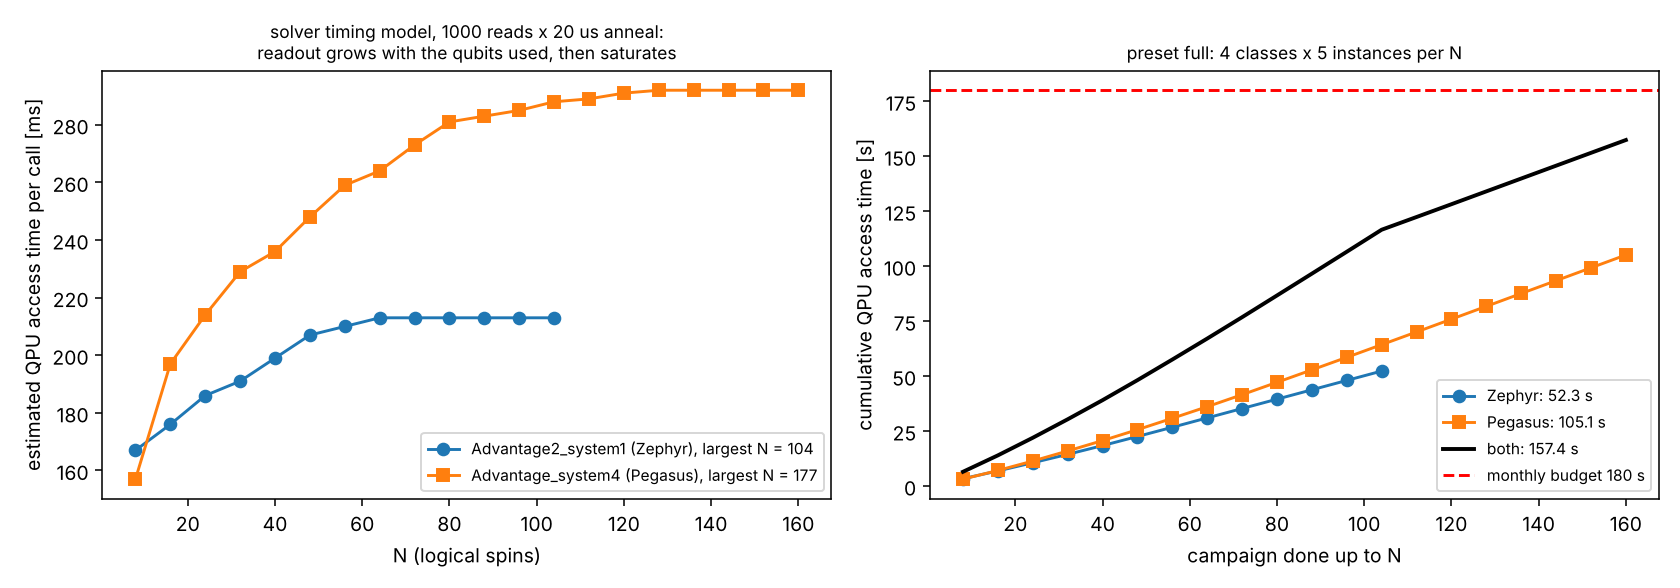
\includegraphics[width=\linewidth]{qpu_check_budget.png}
\caption{Left: estimated access time per call, from your \code{--check}. Right: cumulative budget of the \code{full} campaign: 52.3 s (Zephyr) + 105.0 s (Pegasus) = 157.3 s, against 180 s.}\end{figure}

%=====================================================================================
\section{How QPU time is estimated: three levels}\label{sec:estimate}
%=====================================================================================
\subsection{Level 1: the rough plan (\texorpdfstring{\code{main_simulation.py plan}}{main simulation.py plan})}
For a first idea, before any connection:
\begin{equation}
t_{\rm call}\approx t_{\rm prog}+n_{\rm reads}\,(t_a+t_{\rm ro}+t_d)=15\,{\rm ms}+1000\,(20+100+20)\,\mu{\rm s}=155\,{\rm ms}.
\end{equation}
The constants are generic, and your check shows they \textbf{underestimate}: the real per-call times are 157--292 ms.
Use level 1 only to compare designs, never to spend.

\subsection{Level 2: the solver's timing model (\texorpdfstring{\code{--check}}{--check}, budget guard)}
D-Wave publishes, in each solver's \code{properties["problem_timing_data"]}, the parameters of a model that
\code{estimate_qpu_access_time} evaluates. Reading its source (\code{dwave-cloud-client} 0.14.8) gives
\begin{align}
t_{\rm access}&=\underbrace{t_{\rm prog}^{\rm typ}+t_{\rm prog}^{\rm therm}}_{\text{programming}}
+n_{\rm reads}\Big(t_a+t_{\rm ro}(n_{\rm qubits})+t_{\rm delay}+\max(t_{\rm ro}^{\rm therm},t_{\rm decorr})\Big),\\
t_{\rm ro}(n_{\rm qubits})&=\text{piecewise-linear interpolation (often in log--log) of a measured curve}.
\end{align}
Two consequences, both visible in your check:
\begin{itemize}
\item the cost grows with $N$, because more qubits mean a longer readout, and then \textbf{saturates};
\item Pegasus costs more per call than Zephyr (292 vs 213 ms at large $N$), because its chains use more qubits.
\end{itemize}
Above all, the time is \textbf{proportional to \code{num_reads}} apart from the programming term. Halving the reads roughly halves the budget.

\subsection{Level 3: the charge (\texorpdfstring{\code{qpu_access_time}}{qpu access time})}
After each call the QPU returns its timing. \code{qpu_access_time} is what Leap charges. It is saved in every result
file together with the level-2 estimate (\code{estimated_access_s}), and \code{qpu --spent} sums them and prints the ratio
actual/estimate:
\src{main_simulation.py}{396}{411}{\code{qpu --spent}: what was actually charged}

%=====================================================================================
\section{The budget guard: \texorpdfstring{\code{qpu --budget-seconds S}}{qpu --budget-seconds S}}
%=====================================================================================
\src{main_simulation.py}{312}{343}{budget object and per-call estimate}
\src{main_simulation.py}{346}{394}{the anneal stage: guard before every call, real charge after it}
Rule: before each call, with $\hat t$ the level-2 estimate,
\begin{equation}
\text{call allowed}\iff t_{\rm spent}+f\,\hat t\le S,\qquad f=\max\big(1.5,\ 1.1\cdot\max_{\rm past\ calls}t_{\rm actual}/\hat t\big).
\end{equation}
\begin{itemize}
\item The guard starts with a 50\% safety margin. If the real charges turn out larger than the model, the margin grows automatically.
\item After every call $t_{\rm spent}$ grows by the \emph{real} \code{qpu_access_time}.
\item The budget covers all back-ends of one command (Zephyr, then Pegasus).
\item When a call is refused, the command stops cleanly. Everything done so far is saved, and the same command continues later (resume).
\item Without a timing model (mock QPU) the estimate is a deliberately pessimistic formula: $20\,{\rm ms}+n_{\rm reads}(t_a+300\,\mu{\rm s})$.
\end{itemize}
It is tested in \code{tests/test_campaign.py}: the rule itself, a 0.01 s budget that refuses every call, and a 1 s budget that completes and records estimates.

\paragraph{What the guard cannot guarantee.} It caps the time \emph{this code} spends, using D-Wave's own numbers.
It cannot stop a call once submitted, and it does not see time spent by other programs or other users of the same
Leap project. The Leap dashboard remains the authority on what is left.

%=====================================================================================
\section{From reads to results}
%=====================================================================================
\src{main_simulation.py}{467}{498}{per back-end metrics in \code{collect}}
For each problem class, $N$ and instance $b$, with reference $R_{\rm ref}$ (exact for $N\le24$; otherwise the best of the classical solvers and of every annealer read, polished reads included):
\begin{align}
p_{\rm success}&=\frac{\#\{\text{reads with }R\ge R_{\rm ref}-10^{-9}\}}{n_{\rm reads}}\quad\text{(per read)},\\
\text{residual}&=\frac{R_{\rm ref}-R_{\rm best\ read}}{|R_{\rm ref}|},\\
t_{\rm read}&=\frac{t_{\rm sampling}}{n_{\rm reads}}\quad(t_{\rm sampling}=\text{\code{qpu_sampling_time}}),\\
\text{TTS}_{99}&=t_{\rm read}\,\frac{\ln0.01}{\ln(1-p)}.
\end{align}
\src{main_simulation.py}{517}{532}{time per read and TTS$_{99}$}
\code{compare_backends} ranks the back-ends of the same device for each (class, $N$): higher median $p_{\rm success}$ wins, ties go to the lower residual.
The output is \code{summary/backend_comparison.csv} and \code{.png}.

%=====================================================================================
\section{How the D-Wave path was tested}
%=====================================================================================
\begin{itemize}
\item \code{test_embedding.py}: clique embeddings are valid on both topologies (every chain connected, chains disjoint, every pair linked); Zephyr chains are shorter at production size; the cache round-trips; back-end specs parse; the embedded simulator finds the exact ground state, and the chain strength equals $p\,J_{\rm rms}\sqrt{N-1}$ computed independently.
\item \code{test_campaign.py}: every read is kept and \code{seed} is skipped where unsupported (with \code{ExactSolver}); the whole campaign runs end to end and resumes; \textbf{both QPU back-ends run against \code{MockDWaveSampler}} with Zephyr and Pegasus topologies, using the real \code{DWaveSampler} code path from \code{solver={topology__type}} onwards; the budget guard (rule, refusal, completion, \code{--spent}) is checked.
\item What the mock cannot test: the real timing values, the real noise, SAPI errors and Leap accounting. That is what the one-second test below is for.
\end{itemize}

%=====================================================================================
\section{The one-second test, and a plan for the 180 s}\label{sec:plan}
%=====================================================================================
\subsection{Test: at most 1 s of QPU time, both topologies}
A tiny separate campaign: $N=8$ and $16$, one instance, one problem class, 100 reads per call, both QPUs.
That makes 4 calls. At 100 reads each the timing model gives a few tens of ms per call, so the whole test costs a
fraction of a second. The guard makes \textbf{1 s a hard ceiling} anyway.

\begin{lstlisting}
cd ...\Dimod\src\unlearnable_games_explanation      # (PowerShell, .venv active)
$T = "results\qpu_test"
python main_simulation.py init --preset smoke --out $T --Ns 8,16 --n-instances 1 --regimes sg_satisficing --num-reads 100
python main_simulation.py qpu --out $T --check                  # predicted cost: spends nothing
python main_simulation.py qpu --out $T --budget-seconds 1       # the test: <= 1 s, normally ~0.1-0.2 s
python main_simulation.py qpu --out $T --spent                  # what Leap charged, and actual/estimate
python main_simulation.py classical --out $T                    # seconds, for the reference optimum
python main_simulation.py analyze --out $T                      # success per read, chain breaks
\end{lstlisting}
What to check in the output:
\begin{enumerate}
\item every call prints \code{qpu_access=...ms (est ...ms)}: real vs predicted;
\item \code{--spent}: the total, well below 1 s, and \code{actual/estimate} close to 1;
\item \code{chain_breaks}: should be 0 or tiny at $N=8,16$;
\item the Leap dashboard shows the same usage.
\end{enumerate}

\subsection{Spending the 180 s before 4 November}
Your check gives 157.3 s for the full campaign on both topologies at 1000 reads. That leaves about 22 s of margin,
\emph{if} the real charges match the model, which the test will show. Two safe options:
\begin{table}[H]\centering\small
\begin{tabularx}{\linewidth}{L{4.2cm}L{2.0cm}X}
\toprule
plan & QPU time & comment \\ \midrule
\code{full}, 1000 reads, both QPUs & $\approx157$ s & as designed; run with \code{--budget-seconds 170} so it can never pass 170 s \\
\code{full}, 500 reads (\code{init ... --num-reads 500}) & $\approx80$ s & time $\propto$ reads; leaves $\approx90$ s for a chain-strength scan at the $N$ where success drops \\
\bottomrule
\end{tabularx}
\end{table}
\begin{lstlisting}
$F = "results\full"
python main_simulation.py init --preset full --out $F --force          # (add --num-reads 500 for option 2)
python main_simulation.py qpu --out $F --check
python main_simulation.py qpu --out $F --budget-seconds 170            # stops by itself before 170 s
python main_simulation.py qpu --out $F --spent
\end{lstlisting}
The QPU stage does not need the classical stage. That can run before or after, on the laptop or on Leonardo,
and \code{analyze} combines them. If the run stops on the budget, it has saved everything done so far, and
\code{--spent} shows the total.

%=====================================================================================
\section*{References}
%=====================================================================================
\begin{itemize}
\item D-Wave, Ocean documentation: \url{https://docs.dwavequantum.com/en/latest/ocean/}; Leap authorisation: \url{https://docs.dwavequantum.com/en/latest/ocean/leap_authorization.html}.
\item D-Wave, QPU timing and \code{estimate_qpu_access_time}: \code{dwave.cloud.solver.StructuredSolver} (source read for \S\ref{sec:estimate}, dwave-cloud-client 0.14.8).
\item Boothby, King, Raymond, \emph{Fast clique minor generation in Chimera qubit connectivity graphs}, Quantum Inf.\ Process.\ 15, 495 (2016): the clique embedding.
\item Cai, Macready, Roy, \emph{A practical heuristic for finding graph minors}, arXiv:1406.2741 (2014): minorminer.
\item Cineca, Quantum Computing as a Service: \url{https://www.quantumcomputinglab.cineca.it/en/resources}.
\item Project: \code{Dimod/explanation_project.pdf} (SK game, algorithms, embedding, chains, noise), \code{Dimod/LEAP_TOKEN.md}, \code{README_LOCAL.md}, \code{README_CINECA.md}.
\end{itemize}
\end{document}
